\documentclass[../../main.tex]{subfiles}
\usepackage{pgfplots}
\pgfplotsset{compat=1.17}
\begin{document}
\chapter{Rigging and Layers}
\label{ch:rigging_layers}

In computer graphics, rigging involves setting up a skeletal structure (also known as an armature) that drives the mesh of a character, allowing it to move and deform in a realistic manner. Rigging is a critical component of character animation, as it determines how the character responds to movement and how it deforms during animation. In the context of sign language avatars, rigging plays a crucial role in capturing the complex articulations and expressions of sign language gestures.

The layered approach to rigging, which this chapter explores in depth, offers a sophisticated method for managing these complexities. By dividing the rigging process into several distinct layers—each responsible for a different aspect of the avatar’s movement and deformation—we can achieve a higher level of control and flexibility. This approach not only facilitates the creation of more natural and expressive animations but also makes the system scalable and adaptable to a wide range of linguistic contexts.

In this chapter, we ...todo, section labeled

\section{Procedural Rigging for Signing Avatars}
\label{sec:proc_rig_signing_avatars}

Rigs have been used in computer animation for decades to control the movement and deformation of characters. Traditional rigging systems typically consist of a hierarchical structure of bones, controllers, and constraints that define how the character’s mesh deforms in response to movement. Section {subsubsec:skeleton} in chapter {ch:background_work} gave an overview of the different skeletal structures of an avatar and how it is used to control the character’s movements.

A signing avatar differs significantly from the traditional systems. For starter, no sign language uses the lower body in its articulation. This means that the rigging system for a signing avatar can be simplified to focus on the upper body as shown in figure \ref{ref:upper_body_avatar}. 

\begin{figure}[h]
    \centering
    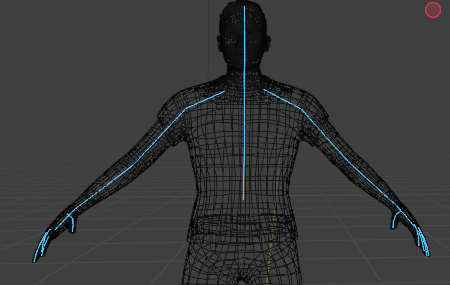
\includegraphics[width=0.5\textwidth]{chapters/rigging_layers/images/upper_body_avatar.png}
    \caption{An example of an upper body avatar rig}
    \label{ref:upper_body_avatar}
\end{figure}

However for procedurally animating a signing avatar, the complexity of sign language gestures and expressions poses unique challenges and necessitates a more sophisticated rigging system.

\subsection{AZee Blender interface}
\label{subsec:azee_blender_interface}

The previous low level synthesizor for AZee \cite{fabrizio} was based on an armature in blender. These bones and sites were mapped to a \emph{SkelSpec} structure. Similarly, AZee's abstract posture was mapped to the \emph{SkelSpec} structure as well. The \emph{SkelSpec} structure thus formed as an intermediate bridge between an Animated AZee Score and the armature \ref{fig:old_interface}. 

\begin{figure}[h]
    \centering
    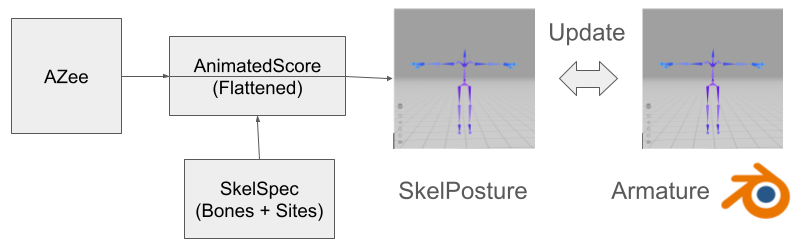
\includegraphics[width=0.5\textwidth]{chapters/rigging_layers/images/old_interface.png}
    \caption{The old interface of the low level synthesizor for AZee}
    \label{fig:old_interface}
\end{figure}

One of the first contributions of my work was to create a new interface for the low level synthesizor for AZee. This new interface didn't have a \emph{SkelSpec} \ref{fig:new_interface} and interacted directly with the blender armature resulting in faster executions \ref{tab:faster_executions}.

\begin{figure}[h]
    \centering
    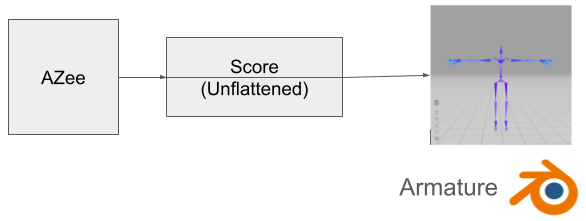
\includegraphics[width=0.5\textwidth]{chapters/rigging_layers/images/new_interface.png}
    \caption{The new interface of the low level synthesizor for AZee}
    \label{fig:new_interface}
\end{figure}

todo
\begin{table}
    \centering
    \begin{tabular}{|c|c|}
        \hline
        \textbf{Interface} & \textbf{Execution time (s)} \\
        \hline
        Old & 0.5 \\
        New & 0.2 \\
        \hline
    \end{tabular}
    \caption{Comparison of execution times between the old and new interfaces}
    \label{tab:faster_executions}
\end{table}

\subsection{Automatic site generation}
\label{subsec:auto_site_generation}

The AZee low-level language consists of 332 sites (appendix \ref{appendix:sites}) which the user to manually create sites in blender. This was a tedious time consuming process process and could lead to errors \ref{fig:prev_sites}.

\begin{figure}[h]
    \centering
    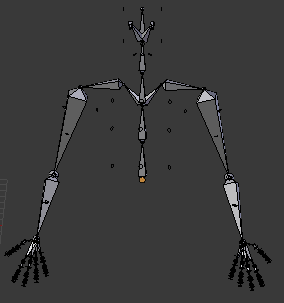
\includegraphics[width=0.5\textwidth]{chapters/rigging_layers/images/prev_sites.png}
    \caption{Manually created sites in the previous low level synthesizor for AZee}
    \label{fig:prev_sites}
\end{figure}

This site generation process could be partially automated if we have the knowledge of the bone structure. Algorithm was used to generate sites based on bone location and avatar mesh using simple raycasting \ref{alg:site_generation_with_raycasting}.

\begin{algorithm}
    \label{alg:site_generation_with_raycasting}
    \caption{Raycasting Algorithm for Automatic Site Generation}
    \begin{algorithmic}
        \State \textbf{Input:} A 3D model with bones
        \State \textbf{Output:} Generated and positioned sites on the model

        \State $sites \gets$ an empty list to store generated site locations

        \State \text{Remove existing sites from the model}

        \State $armature \gets$ find the armature associated with the 3D model

        \For{each $bone$ in $armature$}
            \State $start\_point \gets$ determine a starting point based on the bone's position
            \State $direction \gets$ calculate the direction vector based on the bone's orientation
            
            \State $hit\_success, hit\_location \gets$ perform raycasting from $start\_point$ in $direction$
            \If{$hit\_success$}
                \State $site\_location \gets hit\_location$
            \Else
                \State $site\_location \gets$ fallback location based on predefined logic
            \EndIf

            \State add $site\_location$ to $sites$ list
            
            \State \text{Apply any additional constraints or relationships between the site and the bone}
        \EndFor

        \For{each $finger$ in the model's fingers}
            \For{each $segment$ in $finger$}
                \State repeat the raycasting procedure to determine and store $site\_locations$ for each segment
            \EndFor
        \EndFor

        \State finalize and store the $sites$ list for further processing or rendering
    \end{algorithmic}
\end{algorithm}

The sites an be visualized on the avatar in figure \ref{fig:sites_bazeel_combined}.

\begin{figure}[h]
    \centering
    \begin{subfigure}[b]{0.3\textwidth}
        \centering
        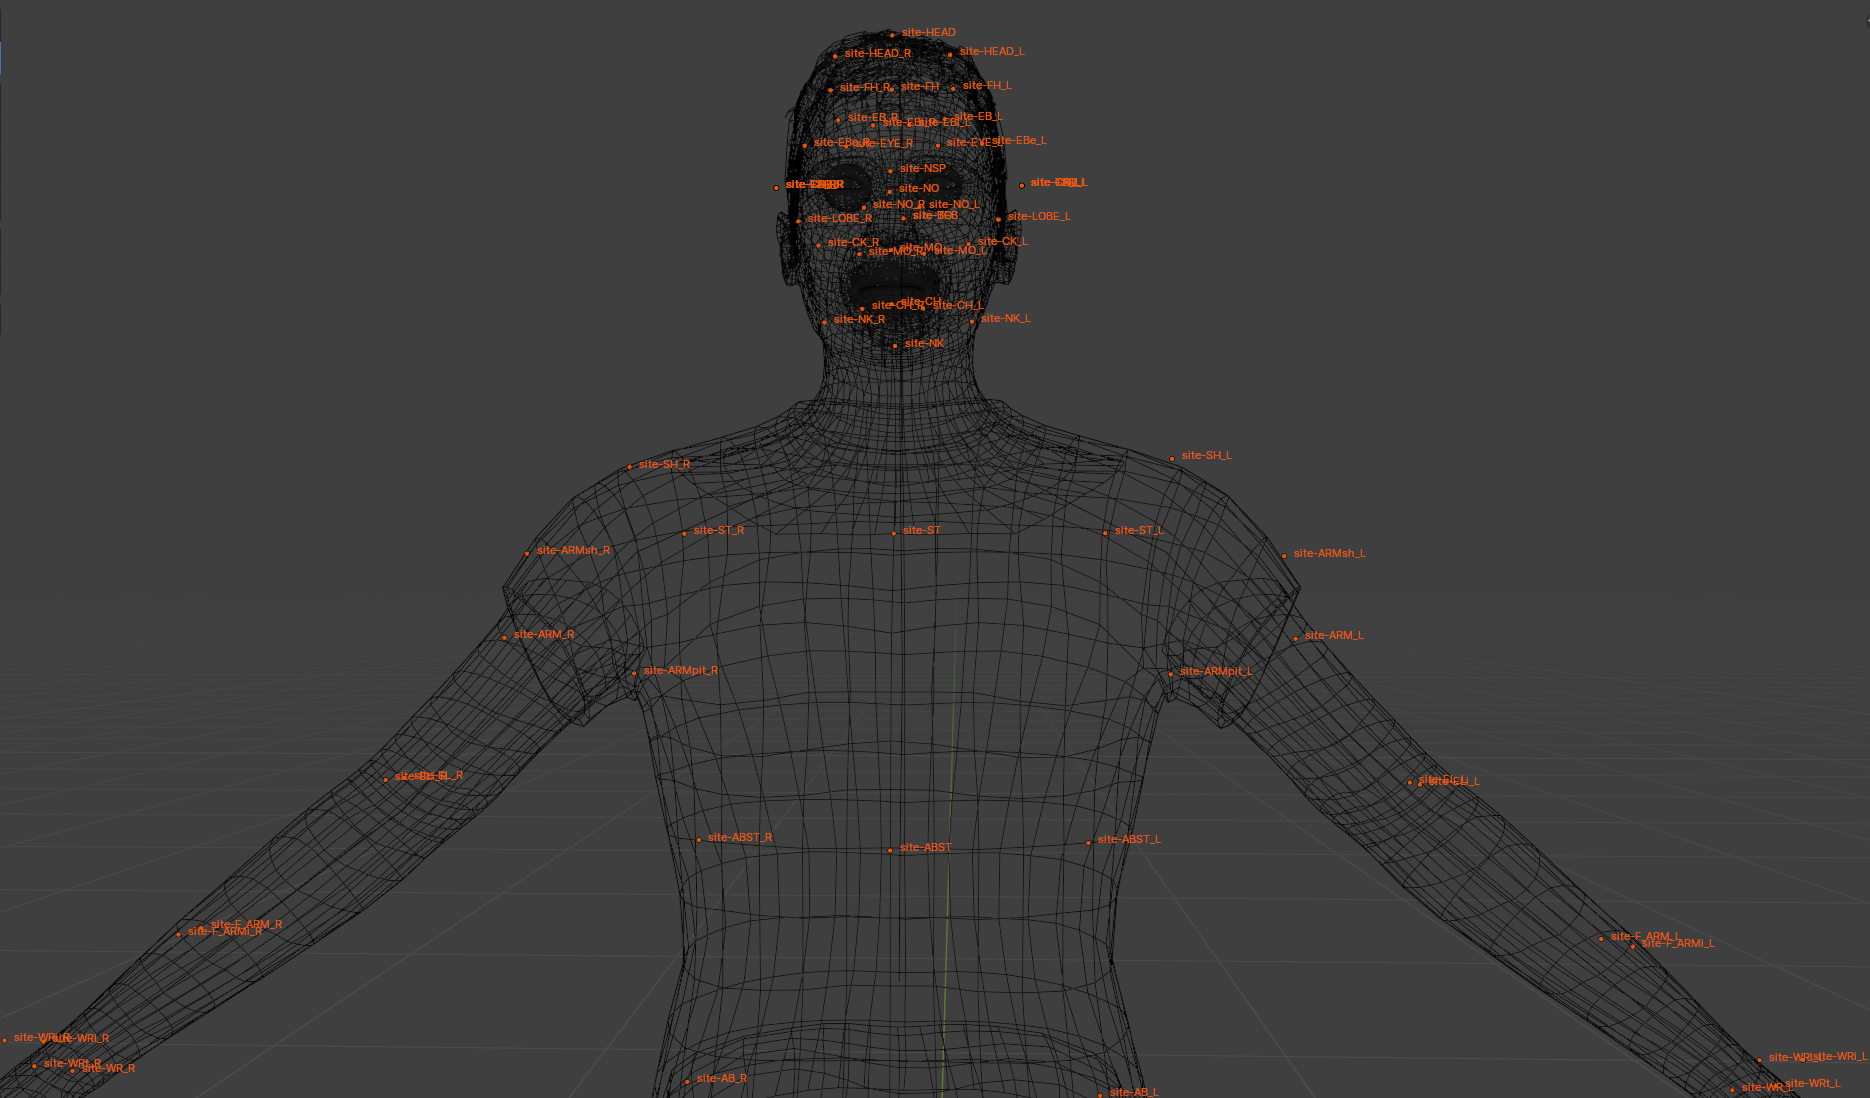
\includegraphics[width=\textwidth]{chapters/rigging_layers/images/sites_body_front.png}
        \caption{Front View of Body Sites}
        \label{fig:sites_body_front}
    \end{subfigure}
    \hfill
    \begin{subfigure}[b]{0.3\textwidth}
        \centering
        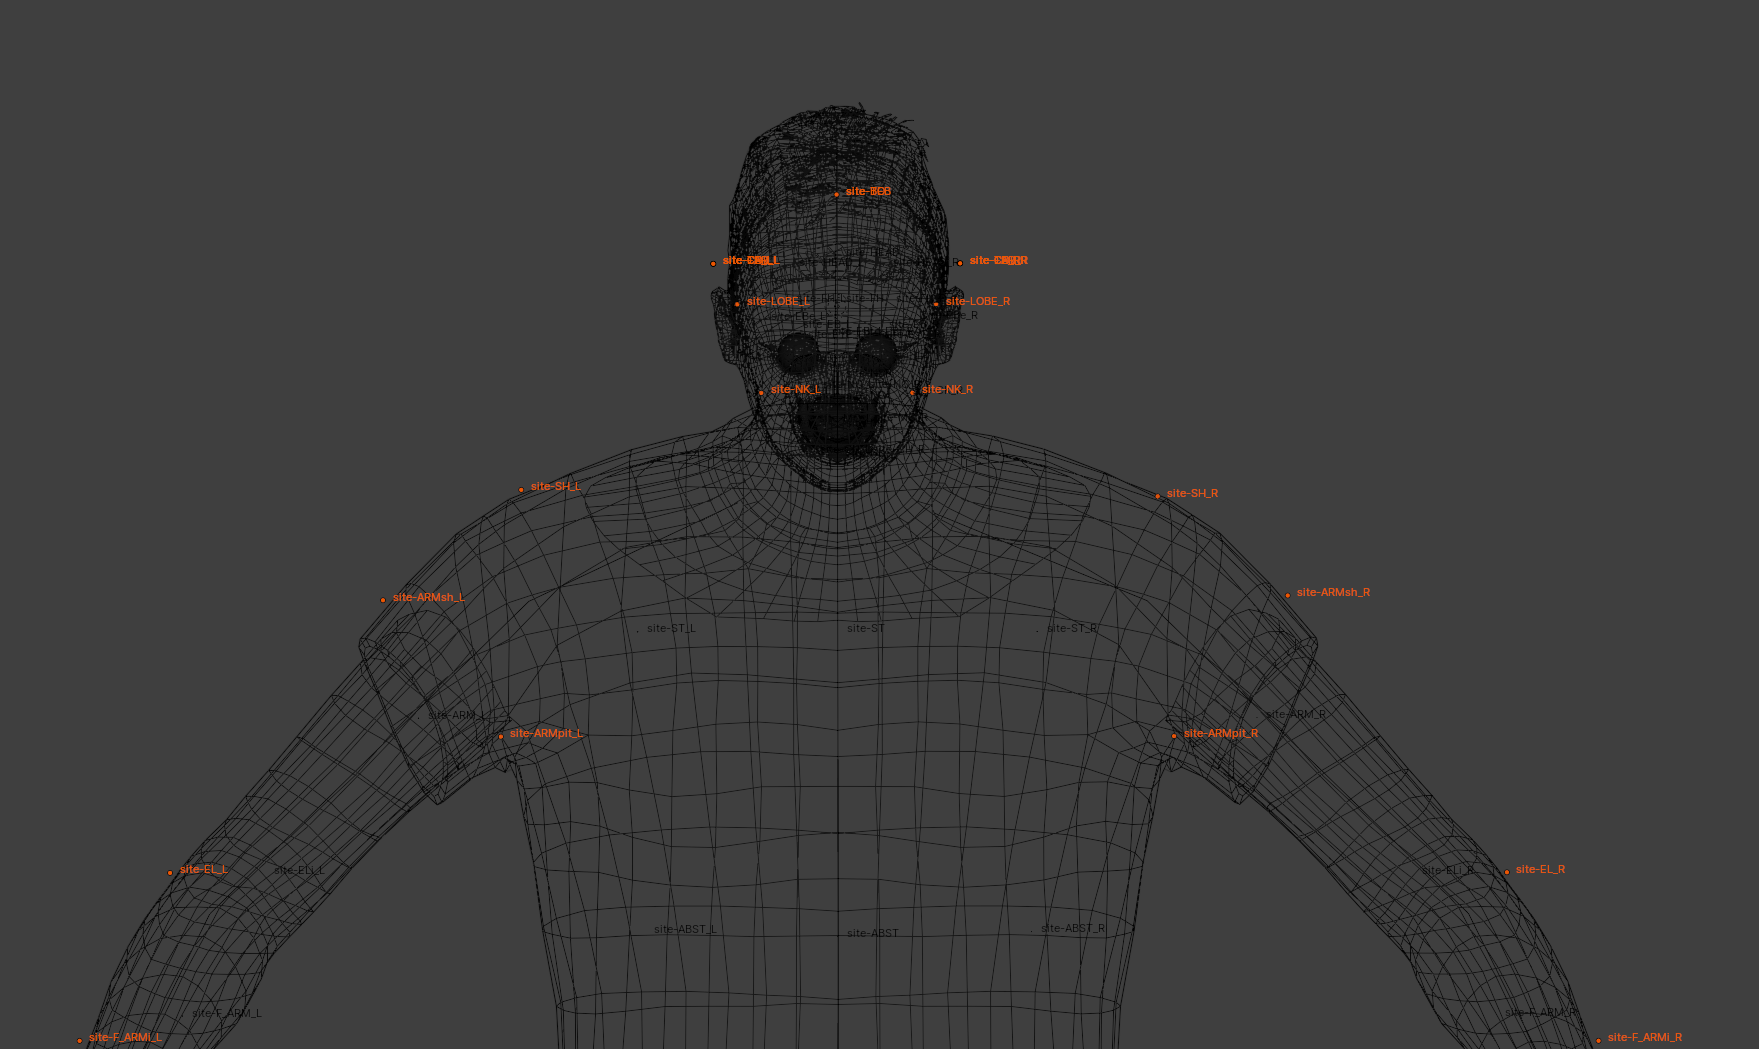
\includegraphics[width=\textwidth]{chapters/rigging_layers/images/sites_body_back.png}
        \caption{Back View of Body Sites}
        \label{fig:sites_body_back}
    \end{subfigure}
    \hfill
    \begin{subfigure}[b]{0.3\textwidth}
        \centering
        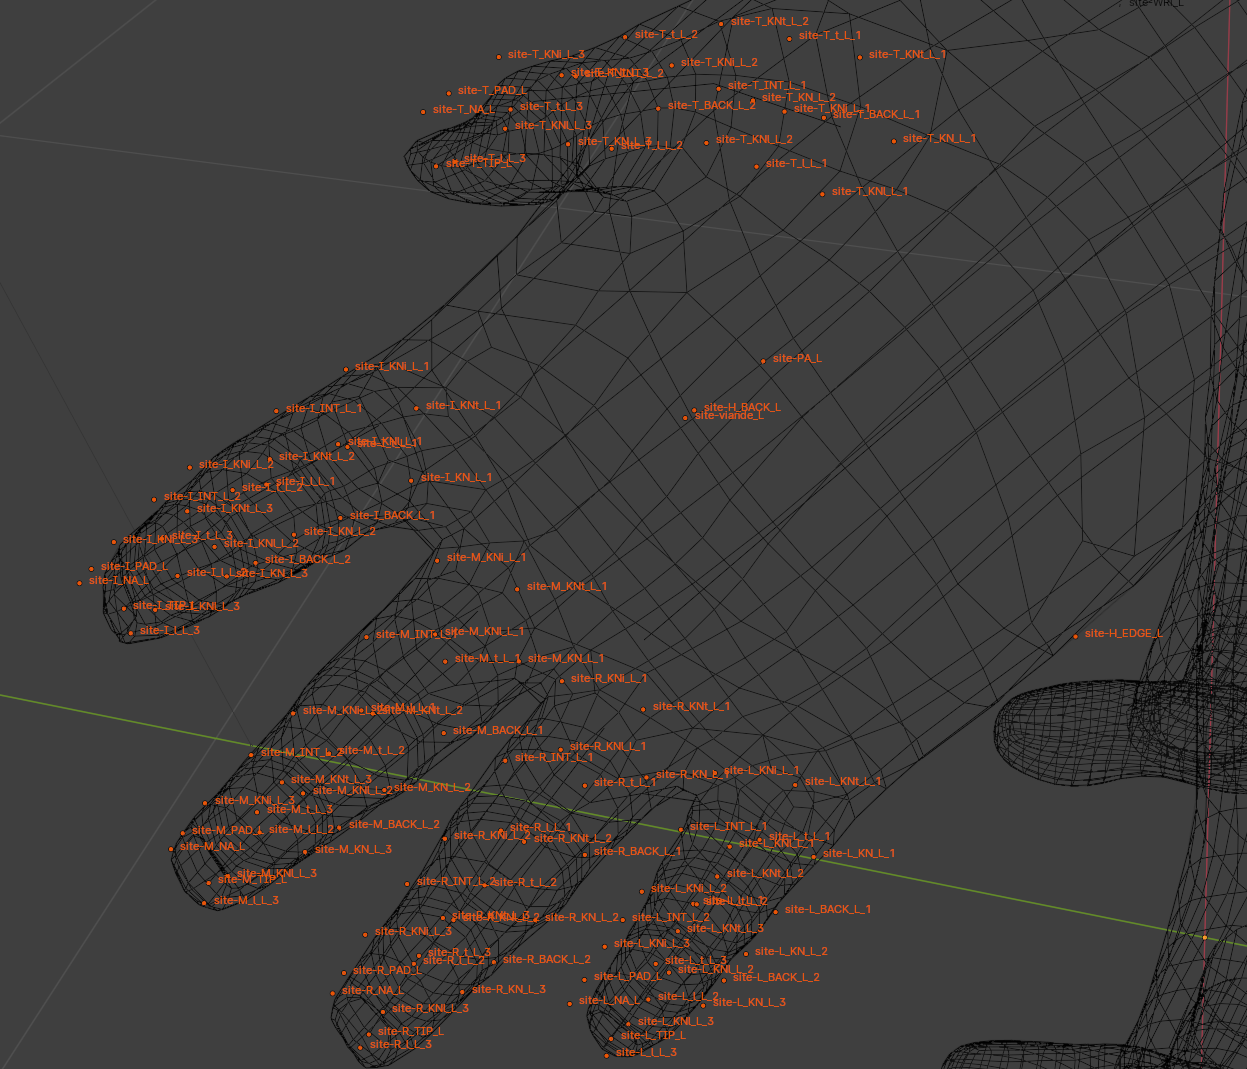
\includegraphics[width=\textwidth]{chapters/rigging_layers/images/sites_hand.png}
        \caption{Hand Sites}
        \label{fig:sites_hand}
    \end{subfigure}
    \caption{AZee sites on the BAZeel avatar: Front and Back Body Views, and Hand Sites}
    \label{fig:sites_bazeel_combined}
\end{figure}


\subsection{Automatic rigging}
\label{subsec:auto_rig}

The previous custom rig contained 57 bones \ref{appendix:old_bone_list}. These bones were initially structured to accommodate the unique skeletal system requirements of the AZee framework, which utilizes a "rotation first" paradigm. However, since Blender operates on a "translation first" paradigm, a conversion process was necessary. This conversion involved splitting each AZee bone into two corresponding Blender bones: one for translation and one for rotation, with the rotation bone named by appending a ".rot" suffix to the original bone name (figure \ref{fig:old_bone_structure}). Additionally, sites were modeled in a dual fashion, where both bones and empty objects were created to manage site positioning and visualization.

\begin{figure}
    \centering
    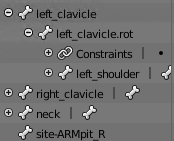
\includegraphics[width=0.5\textwidth]{chapters/rigging_layers/images/old_bone_structure.png}
    \caption{Duplicate bones for rotation and translation}
    \label{fig:old_bone_structure}
\end{figure}

This old system however, can be improved using multiple avatar layers. To do this we need 3 separate layers,

\subsection{Deformation Bone Layer}
\label{subsec:deform_bone_layer}

The deformation bone layer(figure \ref{ref:deform_layer}) is the foundation of the avatar's rig. It includes the bones that directly influence the mesh of the character, controlling how the skin deforms in response to movement. This layer is responsible for the overall shape and posture of the avatar, ensuring that the character's movements are smooth and realistic.

In this layer, the bones are typically organized into a hierarchy, with the root bone controlling the overall position and orientation of the avatar, and child bones controlling specific parts of the body, such as the limbs, spine, and head. Weight painting is used to determine how much influence each bone has over the surrounding mesh, allowing for precise control over how the character's skin deforms.

\begin{figure}
    \centering
    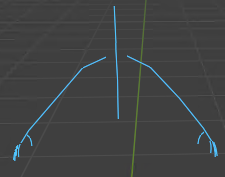
\includegraphics[width=0.5\textwidth]{chapters/rigging_layers/images/deform_layer.png}
    \caption{Deformation bone layer}
    \label{fig:deform_layer}
\end{figure}

\subsection{Inverse Kinematics Layer}
\label{subsec:ik_layer}

The inverse kinematics (IK) layer (figure ref:ik_layer) is responsible for positioning the avatar's limbs and spine by solving for the joint angles required to achieve a desired end-effector position.

A separate IK layers ensures that the FK configuration is not lost during constraint evaluation. If the posture is in IK mode i.e. is solving for a placement, the deform layers copy the orientations resolved by the IK layer.

\begin{figure}
    \centering
    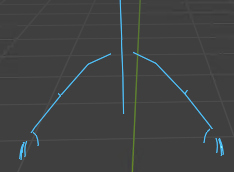
\includegraphics[width=0.5\textwidth]{chapters/rigging_layers/images/ik_layer.png}
    \caption{IK bone layer}
    \label{fig:ik_layer}
\end{figure}

\subsection{Forward Kinematics Layer}
\label{subsec:fk_layer}

The forward kinematics (FK) layer (figure \ref{fig:fk_layer}) controls the rotation of bones in a hierarchical manner, where the rotation of a parent bone affects all its children. This layer is used for broader, more deliberate movements, such as head tilts, body leans, or full-body rotations, which are important for conveying non-manual signals in sign language.

FK provides animators with a high degree of control over each individual bone in the rig, allowing for precise adjustments to the character's pose. Unlike IK, where the position of the end-effector is specified, FK requires the animator to manually rotate each bone in the chain, starting from the root and working down to the extremities. This can be more time-consuming but offers greater flexibility in achieving complex poses.

\begin{figure}
    \centering
    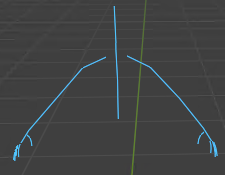
\includegraphics[width=0.5\textwidth]{chapters/rigging_layers/images/fk_layer.png}
    \caption{FK bone layer}
    \label{fig:fk_layer}
\end{figure}

\subsection{Constraint Based Posture Optimization}
\label{subsec:cb_posegen}

The previous low level synthesizor for AZee \cite{fabrizio} used a constraint based optimization algorithm to generate the armature pose for a frame. This algorithm \ref{alg:old_constraint_optimization} collects all posture constaints given by the AZee Animated Score for every frame and solves for the posture by optimizing this constraints using distance functions. 

\begin{algorithm}
    \caption{Constraint-Based Optimization for Posture Synthesis}
    \label{alg:trimmed_constraint_based_optimization}
    \begin{algorithmic}[1]
    \Require $\text{PostureConstraints} \ \mathit{posture\_constraint}$, $\text{Object} \ \mathit{armature\_object}$
    \Ensure Armature object is posed according to the constraints
    
    \State \textbf{Initialize:} $i \gets 0$
    \State $distance\_threshold \gets \mathit{bpy.context.scene.azee\_ik\_site\_distance\_threshold}$
    \State $angle\_threshold \gets \mathit{bpy.context.scene.azee\_ik\_bone\_rot\_angle\_threshold \times \pi / 180}$
    \State $max\_iterations \gets \mathit{bpy.context.scene.azee\_ik\_max\_iterations}$
    
    \While{$i < max\_iterations$}
        \State \textbf{Apply Constraints:} \textsc{ApplyPositionConstraint}($\mathit{posture\_constraint}$), \textsc{ApplyOrientConstraints}($\mathit{posture\_constraint}$)
        \State \textbf{Compute Offsets:} $place\_distance, orient\_angles \gets \textsc{ComputeDistance}(\mathit{posture\_constraint})$
        \If {$\mathit{place\_distance} < \mathit{distance\_threshold}$ \textbf{and} $\max(\mathit{orient\_angles}) < \mathit{angle\_threshold}$}
            \State \textbf{Break:} \textbf{end while}
        \EndIf
        \State $i \gets i + 1$
    \EndWhile
    
    \Procedure{ApplyPositionConstraint}{$\mathit{posture\_constraint}$}
        \If {$\mathit{posture\_constraint.place\_constraint} \neq \text{None}$}
            \State \textbf{Apply IK:} \textsc{ApplyIKConstraint}($\mathit{posture\_constraint.place\_constraint.site\_pose\_bone}$, 
            \textsc{CreateTemporaryTarget}($\mathit{posture\_constraint.place\_constraint.target\_vect}$), \textit{position})
        \EndIf
    \EndProcedure
    
    \Procedure{ApplyOrientConstraints}{$\mathit{posture\_constraint}$}
        \ForAll {$orient\_constraint \in \mathit{posture\_constraint.orient\_constraints}$}
            \State \textbf{Apply IK:} \textsc{ApplyIKConstraint}($orient\_constraint.pose\_bone$, 
            \textsc{CreateTemporaryTarget}($orient\_constraint.get\_target\_quaternion()$), \textit{rotation}, 
            $orient\_constraint.get\_axis\_relaxation\_mask()$)
        \EndFor
    \EndProcedure
    
    \Procedure{ComputeDistance}{$\mathit{posture\_constraint}$}
        \State \Return \textsc{ComputeDistanceFromOffset}(\textsc{ComputePlaceOffset}($\mathit{posture\_constraint}$)), 
        \textsc{ComputeAnglesFromOffsets}(\textsc{ComputeOrientOffsets}($\mathit{posture\_constraint}$))
    \EndProcedure
    \end{algorithmic}
\end{algorithm}

The approach handles only placements and orientations and uses a flattened animated AZee Score. This was improved \ref{alg:new_constraint_optimization} by generating from the multi-track synced score itself(more discussed in chapter \ref{ch:multi-track}) with support for other constraints such as \emph{morph}, \emph{lookat} and \emph{trill}.

\begin{algorithm}
    \caption{Constraint-Based Optimization for Posture Synthesis}
    \label{alg:trimmed_multi_track_optimization}
    \begin{algorithmic}[1]
        \Require $\text{PostureConstraints} \ \mathit{posture\_constraint\_DAG}$, $\text{Object} \ \mathit{armature\_object}$, $\text{FrameRange} \ \mathit{frames}$
        \Ensure Armature object is posed according to the constraints
        
        \State \textbf{Initialize:} $i \gets 0$
        \State $distance\_threshold \gets \mathit{bpy.context.scene.azee\_ik\_site\_distance\_threshold}$, $angle\_threshold \gets \mathit{bpy.context.scene.azee\_ik\_bone\_rot\_angle\_threshold \times \pi / 180}$
        \State $max\_iterations \gets \mathit{bpy.context.scene.azee\_ik\_max\_iterations}$
        \State $\mathit{sorted\_constraints} \gets \mathit{posture\_constraint\_DAG.topological\_sort()}$
        \State $frames\_to\_keyframe \gets \textsc{DetermineFramesToKeyframe}(\mathit{frames}, \mathit{dynamic\_points})$
        
        \While{$i < max\_iterations$}
            \ForAll {$f \in \mathit{frames\_to\_keyframe}$}
                \State $\mathit{cumulative\_loss} \gets 0.0$
                \ForAll {$constraint \in \mathit{sorted\_constraints}$}
                    \State \textbf{Apply Constraint:} \textsc{ApplyConstraint}($constraint$, $f$)
                    \State $\mathit{cumulative\_loss} \gets cumulative\_loss + \mathit{constraint.get\_loss(f)}$
                \EndFor
                \If {$cumulative\_loss < \mathit{bpy.context.scene.azee\_animator\_threshold}$}
                    \State \textbf{Break:} \textbf{end while}
                \EndIf
                \State \textbf{Insert Keyframe:} \textsc{InsertKeyframe}($f$)
            \EndFor
            \State $i \gets i + 1$
        \EndWhile
        
        \Procedure{ApplyConstraint}{$constraint, frame$}
            \If {$constraint$ \textbf{is} PlacementConstraint}
                \State \textsc{PlaceSite}($constraint.site$, \textsc{EvaluatePlacementTarget}($constraint$, $frame$))
            \ElsIf {$constraint$ \textbf{is} OrientationConstraint}
                \State \textsc{RotateBone}($constraint.bone$, \textsc{EvaluateOrientation}($constraint$, $frame$))
            \ElsIf {$constraint$ \textbf{is} MorphConstraint}
                \State \textsc{ApplyMorph}($constraint$, $frame$)
            \ElsIf {$constraint$ \textbf{is} LookAtConstraint}
                \State \textsc{RotateEyesToTarget}($constraint.eyes$, \textsc{EvaluateLookAtPoint}($constraint$, $frame$))
            \ElsIf {$constraint$ \textbf{is} TrillConstraint}
                \State \textsc{ApplyTrill}($constraint$, $frame$)
            \ElsIf {$constraint$ \textbf{is} TranspathConstraint}
                \State \textsc{FollowPath}($constraint.site$, \textsc{DeterminePath}($constraint$, $frame$))
            \Else
                \State \textsc{HandleError}()
            \EndIf
        \EndProcedure
        
        \Procedure{DetermineFramesToKeyframe}{$frames, dynamic\_points$}
            \State \Return $\textsc{IdentifyKeyFrames}(\mathit{frames}) \cup \textsc{DynamicFrameRanges}(dynamic\_points)$
        \EndProcedure
        
        \Procedure{InsertKeyframe}{$frame$}
            \ForAll {$fcurve \in \mathit{armature\_object.animation\_data.action.fcurves}$}
                \State \textsc{KeyframeInsert}($fcurve$, $frame$)
            \EndFor
        \EndProcedure
    \end{algorithmic}
\end{algorithm}

\subsection{Morphs Constraints}
\label{subsec:morph_constraints}

The word "morph" comes from the Greek word "morphē" (μορφή), which means "form" or "shape." In modern usage, "morph" is often used as a shorthand for "morphing". In the field of computer graphics and animation, morphs are predefined shape keys that modify the mesh of the avatar independently of the skeletal structure, allowing for the detailed control of specific aspects of the avatar's appearance that cannot be easily achieved through bone manipulation alone. This includes subtle facial expressions, muscle bulges, and other nuanced gestures that are critical for conveying meaning in sign language.

AZee sees morphs as any change in the configuration of the avatar, which can be specified by the linguist in 1 dimension. For instance, closing of hands(a change in skeleton configuration) or raising the eyebrows(a change in the 3D mesh). Thus, these changes could also be formalized as Pose-Space Deformations.

\subsubsection{Skeletal Morphs}
\label{subsec:skel_morphs}

Morph targets are typically generated by sculpting the avatar's mesh into various shapes that correspond to different expressions or gestures. These sculpted shapes are then saved as "keys," which can be blended together during animation to produce the desired expression. This process allows for a high degree of flexibility in animation, as different keys can be combined in real-time to create a wide range of expressions.

For example, in a signing avatar, a morph might be used to raise one eyebrow while simultaneously forming a specific hand shape. The morph layer interacts with the skeletal layer by adjusting the mesh deformation in response to the skeletal movements, ensuring that the overall appearance of the avatar remains cohesive. This interaction is crucial for maintaining the realism of the avatar, as it allows for natural transitions between different expressions and gestures.

\subsubsection{Facial Morphs}
\label{subsubsec:facial_morphs}

Morphs do not operate in isolation but rather work in tandem with the avatar's skeletal movements. While the skeletal system provides the foundation for the avatar's overall posture and major movements, morphs add an additional layer of detail by refining the surface deformations of the mesh. This is particularly important in sign language synthesis, where both gross motor movements and fine motor expressions must be synchronized to convey meaning accurately.

For instance, when an avatar raises its hand to sign, the skeletal system dictates the overall arm movement, but the morphs refine the finger positions and facial expressions, ensuring that the sign is communicated effectively. The ability to blend morphs with skeletal movements allows for the creation of more natural and fluid animations, which are essential for the realism and believability of the avatar.

\subsubsection{1D Space of a Morph}
\label{subsubsec:morph_space}

todo
- show morph space
- show and explain graph

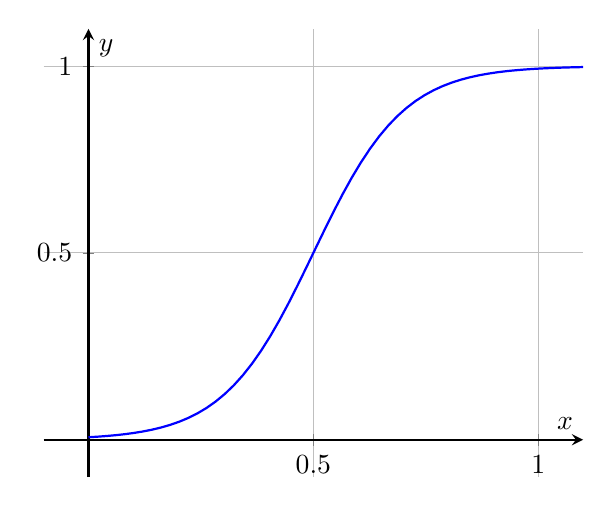
\begin{tikzpicture}
    \label{fig:morph_graph}
    \begin{axis}[
        domain=0:2, % Define the range of x
        samples=100, % Number of samples to plot
        axis lines=middle, % Draw the axes in the middle
        xlabel={$x$},
        ylabel={$y$},
        ymin=-0.1, ymax=1.1, % Define y-axis range
        xmin=-0.1, xmax=1.1, % Define x-axis range
        xtick={0, 0.5, 1, 2},
        ytick={0, 0.5, 1},
        grid=both, % Add a grid
        thick,
    ]
    \addplot[blue, thick] {1 / (1 + exp(-10 * (x - 0.5)))};
    \end{axis}
\end{tikzpicture}

\subsubsection{Integration with other layers}
\label{subsubsec:intergation}

todo
\begin{algorithm}
    \caption{Posture Generation with Constraints}
    \label{alg:posture_morph_integrate}
    \begin{algorithmic}[1]    
    \Procedure{GeneratePosture}{$Blocks$}
        \For{each $Block$ in $Blocks$}
            \State $Constraints \gets \text{TopologicalSort}(\text{CreateDAG}(Block))$
            \For{each $Frame$ from $Block.Start$ to $Block.End$}
                \For{$Epoch \gets 1$ to $MaxEpochs$}
                    \State $Loss \gets 0$
                    \For{each $C$ in $Constraints$}
                        \State \text{Apply}($C$, $Frame$)
                        \State $Loss \gets Loss + \text{ComputeLoss}(C, Frame)$
                    \EndFor
                    \If{$Loss < Threshold$} \textbf{break} \EndIf
                \EndFor
                \State \text{InsertKeyframe}(Frame)
            \EndFor
        \EndFor
    \EndProcedure
    
    \Procedure{Apply}{$C$, $Frame$}
        \If{$C$ is $MorphConstraint$} \State \text{ApplyMorph}($C$, $Frame$)
        \ElsIf{$C$ is $PlacementConstraint$} \State \text{ApplyPlacement}($C$, $Frame$)
        \ElsIf{$C$ is $OrientationConstraint$} \State \text{ApplyOrientation}($C$, $Frame$)
        \EndIf
    \EndProcedure
    
    \end{algorithmic}
\end{algorithm}

todo
\begin{algorithm}
    \caption{Calculate MorphConstraint Loss in Terms of FK}
    \begin{algorithmic}[1]
        \label{alg:morph_constraint_loss}
    \Procedure{ComputeMorphFKLoss}{$\mathbf{p}_{\text{current}}$, $\mathbf{p}_{\text{target}}$, $\mathbf{q}_{\text{current}}$, $\mathbf{q}_{\text{target}}$}
        \State $\text{PositionLoss} \gets \|\mathbf{p}_{\text{current}} - \mathbf{p}_{\text{target}}\|$
        \State $\text{RotationDiff} \gets \mathbf{q}_{\text{current}} \cdot \mathbf{q}_{\text{target}}$
        \State $\text{RotationLoss} \gets 1 - |\text{RotationDiff}|$
        \State $\text{TotalLoss} \gets \lambda_p \times \text{PositionLoss} + \lambda_r \times \text{RotationLoss}$
        \State \Return $\text{TotalLoss}$
    \EndProcedure
    
    \Procedure{ApplyMorphConstraint}{$\text{MorphConstraint}$, $\text{Frame}$}
        \State $\mathbf{p}_{\text{current}}, \mathbf{q}_{\text{current}} \gets \text{ApplyMorph}(\text{MorphConstraint}, \text{Frame})$
        \State $\mathbf{p}_{\text{target}}, \mathbf{q}_{\text{target}} \gets \text{GetTargetState}(\text{Frame})$
        \State $\text{Loss} \gets \text{ComputeMorphFKLoss}(\mathbf{p}_{\text{current}}, \mathbf{p}_{\text{target}}, \mathbf{q}_{\text{current}}, \mathbf{q}_{\text{target}})$
        \State \Return $\text{Loss}$
    \EndProcedure
    
    \end{algorithmic}
\end{algorithm}

\section{Results}
\label{sec:results}
todo The implementation of the layered rigging system in Blender has yielded promising results in the synthesis of sign language animations. By leveraging the strengths of both procedural and data-driven techniques, we have been able to create animations that are both natural and scalable.

\subsection{Performance and Scalability}
TODO: Discuss the performance of the system in terms of processing time, memory usage, and scalability. Explain how the system handles complex utterances and large datasets.

\subsection{Quality of Animation}
todo The quality of the animations produced by the system has been evaluated based on several criteria, including the naturalness of movement, the accuracy of the gestures, and the expressiveness of the avatar. Preliminary results indicate that the system is capable of producing high-quality animations that closely match the intended linguistic meaning.

\section{Discussion}
todo The layered approach to rigging provides a robust framework for synthesizing sign language animations that are both flexible and natural. By dividing the rigging process into distinct layers, each responsible for different aspects of the avatar's movement, we can achieve a high level of control over the final animation. This modular approach also makes it easier to integrate new techniques and technologies as they become available.

\subsection{Comparison with Other Methods}
TODO: Compare the layered approach with other rigging and animation methods used in sign language synthesis. Discuss the advantages and disadvantages of each approach.

\subsection{Challenges and Limitations}
todo While the layered approach offers many benefits, it also presents certain challenges. Managing the interactions between layers can be complex, particularly when dealing with highly articulated movements or subtle expressions. Additionally, the system requires careful tuning to ensure that the animations remain cohesive and natural.

todo Another limitation is the reliance on pre-recorded motion data for certain aspects of the synthesis. While this data enhances the realism of the animations, it also introduces dependencies on the quality and diversity of the recorded dataset. Future work will focus on improving the integration of procedural and data-driven techniques to minimize these dependencies.

\section{Future Work}
todo tangent space stuff The research and development of this layered rigging system is ongoing, with several avenues for future exploration.

\subsection{Enhancing Naturalness}
TODO: Explore advanced techniques for improving the naturalness of the animations, such as the use of noise functions, machine learning models for motion prediction, and real-time adjustments to the rig based on user input.

\subsection{Integration with Other Technologies}
TODO: Investigate the integration of the rigging system with other technologies, such as virtual reality (VR), augmented reality (AR), or real-time motion capture, to expand its applications.

\section{Conclusion}
todo The development of a layered rigging system for sign language avatars represents a significant step forward in the field of sign language synthesis. todo

\end{document}